\begin{figure}[ht]
    \centering
    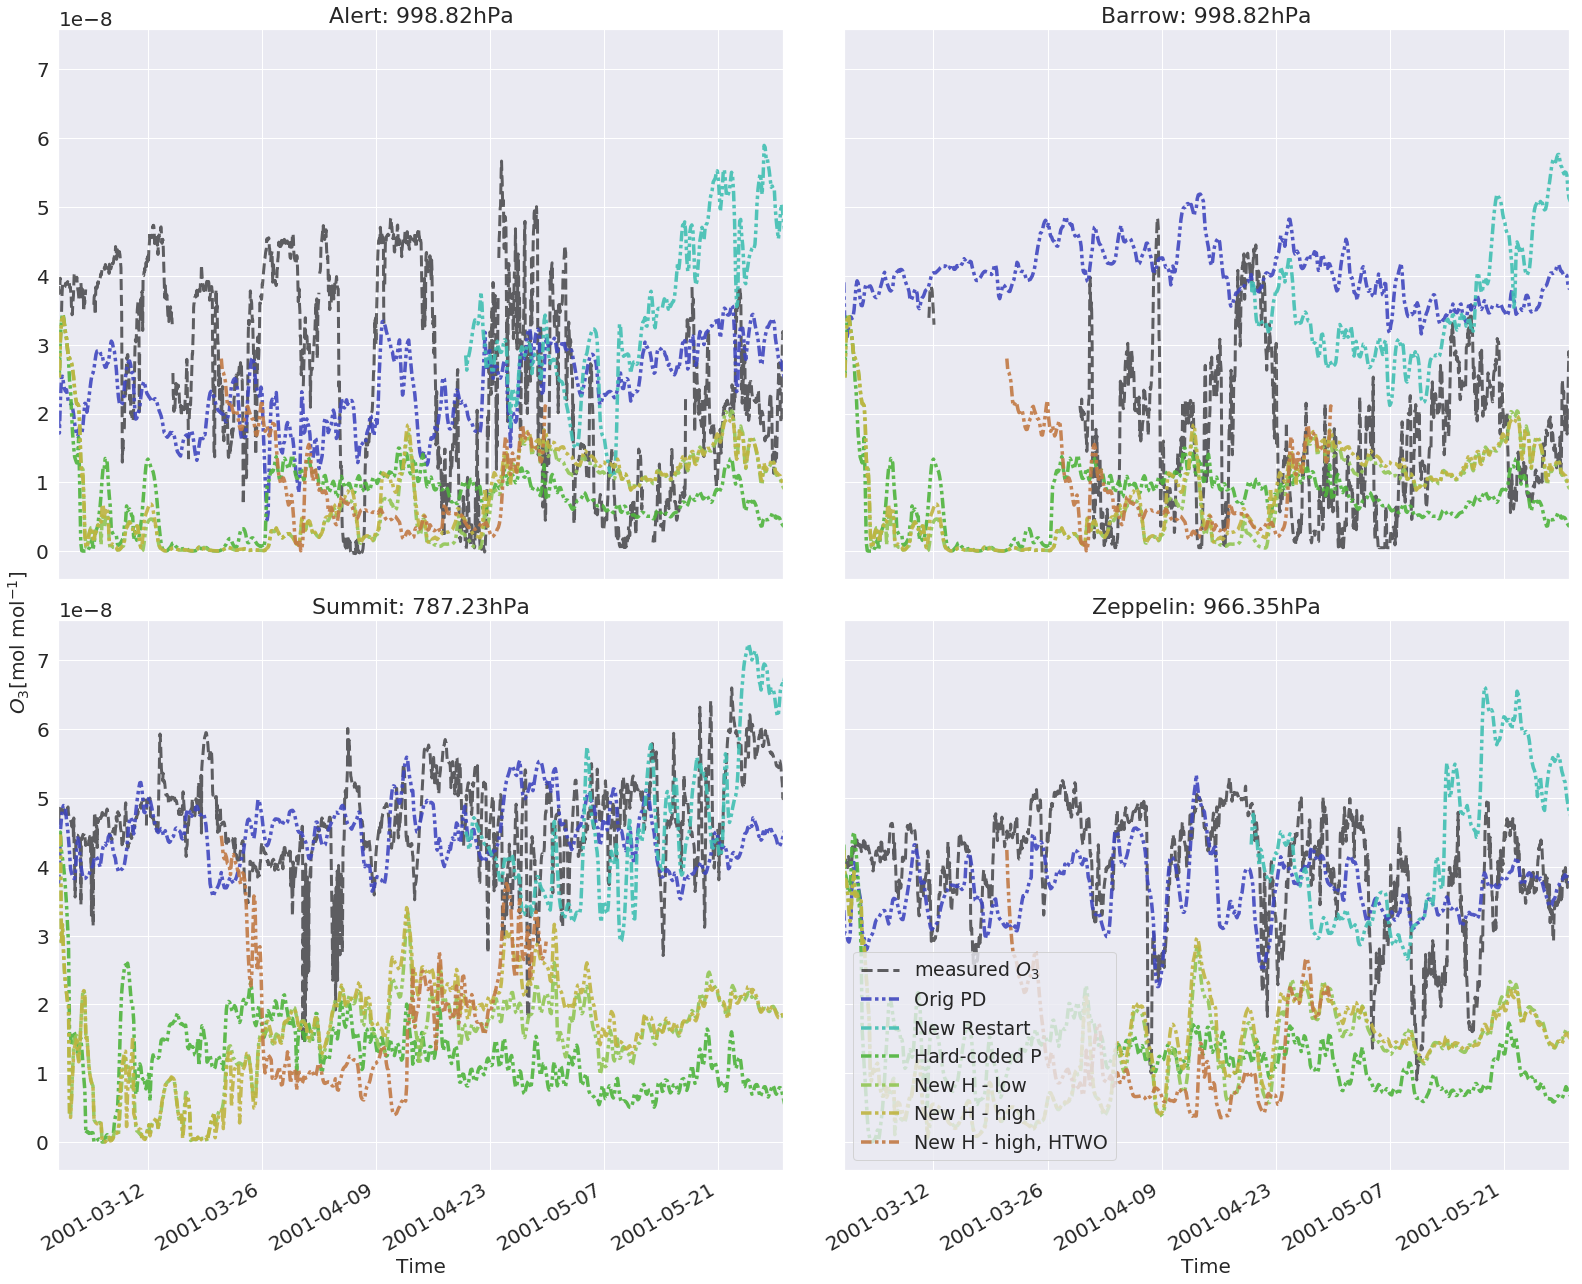
\includegraphics[width=\linewidth]{Chapter6_Results/images/ozone_stationComp_2001/ozone_2001_step3.png}
    \caption{Ozone measurements (black line) and model results from the original CTM3 (blue line) (these two are the same as in Figure \ref{fig:CompObsOrigBE}), test with new restart file from Section \ref{sec:res_step2} (turquoise line), hard-coded photodissociation rates (green line), new (low) Henry's law constant of $7.2\times10^{-1} M atm ^{-1}$ and $6100 K$ (light green line), new (high) Henry's law constant of $2.5\times10^{1} M atm ^{-1}$ and $370 K$ (yellow line) and the latter ran at \texttt{HTWO} resolution (orange line) at the four different stations, Alert (top left), Barrow (top right), Summit (lower left) and Zeppelin (lower right) with available measurements in 2001. Model results were taken from the approximate altitude of the station in hPa \protect\footnotemark}
    \label{fig:ozone_2001_step3}
\end{figure}

\footnotetext{H = Henry's Law}